\section{Related Work}

\textbf{\textit{A. Task Offloading in Vehicular Networks}}

Existing V2X offloading approaches broadly include heuristic, optimization-based, and learning-based methods. Greedy and heuristic schemes such as CoopEC~\cite{shao2025} select offloading destinations using predefined decision rules, but their ability to adapt to rapidly varying channel conditions and shared-resource contention is limited. Bandit and tabular approaches such as UCB~\cite{wu2021} introduce online adaptation but are better suited to relatively small and stationary decision spaces. Control-theoretic methods based on Lyapunov optimization~\cite{jing2019} explicitly address queue stability, but generally optimize time-averaged objectives rather than task-specific deadline compliance. Deep reinforcement learning approaches~\cite{jing2019,yun2022,lowe2017} provide greater adaptability, although many existing formulations simplify either the communication interface or the computation decision through single-RAT operation or binary local/offload actions.

Guo et al.~\cite{guo2026} proposed DTOF/HIOA, combining DDQN+LSTM with Nash-equilibrium-based optimization in a three-tier cloud-edge-vehicle architecture over 5G-NR. Although the framework achieves strong delay performance, it does not jointly consider heterogeneous RAT selection, federated cooperation, and shared RSU queue contention across co-located vehicles.

A complementary line of work considers partial offloading, where a task is divided between local and MEC execution rather than being processed entirely at one location. Parallel local and remote execution can reduce completion time by exploiting both computing resources simultaneously. Prior work has established such parallel-execution models~\cite{mao2017}, including formulations in which total completion delay is governed by the slower of the local and remote processing branches. In most such approaches, however, the offload ratio is optimized independently of heterogeneous radio selection. MA-ROPE instead couples these decisions: the amount of computation transmitted and the RAT used for transmission are jointly determined, with the realized offload ratio adapting to the SINR of the selected interface.

\textbf{\textit{B. Multi-RAT and Heterogeneous Access Selection}}

Heterogeneous V2X access has traditionally been studied primarily as a communication-selection problem. Yacheur et al.~\cite{yacheur2023} developed DDQN-based selection between ITS-G5 and LTE-V2X, demonstrating the benefit of adapting RAT choice to channel conditions. Their physical-layer parameters and SINR-based Division Mode motivate elements of the heterogeneous channel and partial-offloading models adopted in MA-ROPE.

More recent work has expanded heterogeneous access beyond two interfaces. Xiong et al.~\cite{xiong2021} investigated federated Q-learning over three RATs, while other studies consider multi-RAT assignment and heterogeneous V2X resource allocation across combinations such as DSRC, cellular V2X, and mmWave. Mirza et al.~\cite{mirza2023} proposed the MCLA framework for heterogeneous 5G-NR-V2X edge networks, incorporating mobility, contact duration, MEC load awareness, and task partitioning. Their scheme supports load-aware server selection and partial execution, but uses model-based decision logic rather than a learned federated joint RAT--offload policy.

These studies establish the value of heterogeneous access, but their decision structures remain different from the problem addressed here. RAT-selection methods generally determine the interface over which an already-defined workload is transmitted, whereas computation offloading must additionally determine how much workload should be transmitted. The two decisions interact directly because the selected RAT affects transmission latency and reliability, while the offloaded fraction determines transmission duration, energy consumption, local computation demand, and MEC load.

MA-ROPE therefore represents RAT identity and workload partitioning within a common decision process rather than optimizing them as separate stages.

\textbf{\textit{C. Federated and Privacy-Preserving Learning for VEC}}

Cooperative learning has increasingly been applied to vehicular edge resource management. Centralized multi-agent approaches such as MADDPG~\cite{lowe2017} can exploit joint agent information during training and provide strong coordination, but require centralized access to information that remains local under a federated formulation.

Federated learning offers an alternative by aggregating model parameters rather than centrally collecting each vehicle's training observations. Moon and Lim~\cite{moonlim2022} proposed federated DDPG for vehicular edge task offloading and power control, combining local actor-critic learning with periodic model aggregation. Their formulation incorporates queue information and power control, but does not perform heterogeneous RAT selection or explicit partial-offload-ratio selection. Other recent federated VEC approaches employ DDQN or multi-agent DRL with FedAvg for collaborative offloading, but similarly focus on destination or mode selection rather than a joint RAT--partial-offload action.

Importantly, heterogeneous RAT selection and federated learning have also previously been combined. Xiong et al.~\cite{xiong2021}, for example, use federated Q-table averaging for selection among three RATs. Their framework demonstrates that federated learning can coordinate heterogeneous access decisions, but it remains tabular and does not incorporate partial workload execution or explicit shared MEC queue dynamics.

Accordingly, the contribution of MA-ROPE is not simply the combination of federated learning and multi-RAT access. Rather, FedAvg is applied to a policy whose decision space jointly captures heterogeneous RAT selection, workload partitioning, and queue-aware offloading.

The privacy benefit should also be interpreted carefully. FedAvg avoids centralized pooling of raw observations, but exchanging model updates does not itself provide formal privacy guarantees because trained parameters may remain vulnerable to inference attacks~\cite{zhu2019}. Secure aggregation and differential privacy are therefore complementary mechanisms for production deployment.

\textbf{\textit{D. Research Gap}}

The literature demonstrates substantial progress in each component of vehicular edge offloading, but these components are predominantly addressed in isolation. DRL-based offloading commonly simplifies the communication interface; partial-offloading methods optimize workload partitioning without jointly selecting among heterogeneous V2X RATs; multi-RAT approaches select interfaces without jointly learning partial execution under shared MEC contention; and federated VEC methods enable distributed cooperative learning without incorporating the complete joint RAT--partial-offloading decision.

Existing studies come close along individual dimensions. Prior work includes federated multi-RAT selection~\cite{xiong2021}, heterogeneous V2X task offloading with up to three RATs~\cite{mirza2023}, federated DRL for edge resource management~\cite{moonlim2022}, and partial computation offloading~\cite{mao2017}. The literature nevertheless indicates that these capabilities have not been jointly represented in a unified policy that combines heterogeneous RAT choice, partial workload execution, explicit shared RSU queue contention, and federated deep reinforcement learning.

MA-ROPE addresses this interaction by jointly selecting the communication interface and partial-offload decision while accounting for heterogeneous channel conditions and shared RSU queue state, with cooperative policy learning through FedAvg. This formulation enables the central question considered in this work: whether deadline-compliant delivery can be preserved as fleet density and shared MEC contention increase. Table I summarizes the positioning of MA-ROPE relative to representative prior approaches.

\begin{table}[htbp]
\caption{Literature Comparison --- Feature Coverage}
\label{tab:literature}
\centering
\resizebox{\columnwidth}{!}{%
\begin{tabular}{|l|c|c|c|c|c|c|}
\hline
\textbf{Paper} & \textbf{Multi-RAT} & \textbf{Partial $\rho$} & \textbf{Queue Cont.} & \textbf{FL Privacy} & \textbf{Jakes} & \textbf{Yacheur Ch.} \\
\hline
Guo 2026~\cite{guo2026} & $\times$ & Partial & Per-node & $\times$ & $\times$ & $\times$ \\
Yacheur 2023~\cite{yacheur2023} & \checkmark ITS+LTE & $\times$ & $\times$ & $\times$ & \checkmark & \checkmark \\
Shao 2025~\cite{shao2025} & $\times$ & $\times$ & $\times$ & \checkmark FedAvg & $\times$ & $\times$ \\
Wu 2021~\cite{wu2021} & $\times$ & $\times$ & $\times$ & $\times$ & $\times$ & $\times$ \\
\textbf{MA-ROPE (ours)} & \textbf{\checkmark 4 RATs} & \textbf{\checkmark $\rho\in\{0..1\}$} & \textbf{\checkmark shared RSU} & \textbf{\checkmark FedAvg} & \textbf{\checkmark Jakes} & \textbf{\checkmark adopted} \\
\hline
\end{tabular}%
}
\end{table}

\subsection{Contribution Decomposition}

Fig. 1 decomposes MA-ROPE utility into per-component contributions for the N=8 reference setting retained for v10 compatibility. Starting from AllOffload (U=0.8166), adding shared-queue awareness, multi-RAT selection, DRL policy, and FedAvg yields MA-ROPE (U=0.8443). The primary dense-fleet results are reported separately at N=32 in Table IV and Table V.

\begin{figure}[htbp]
\centering
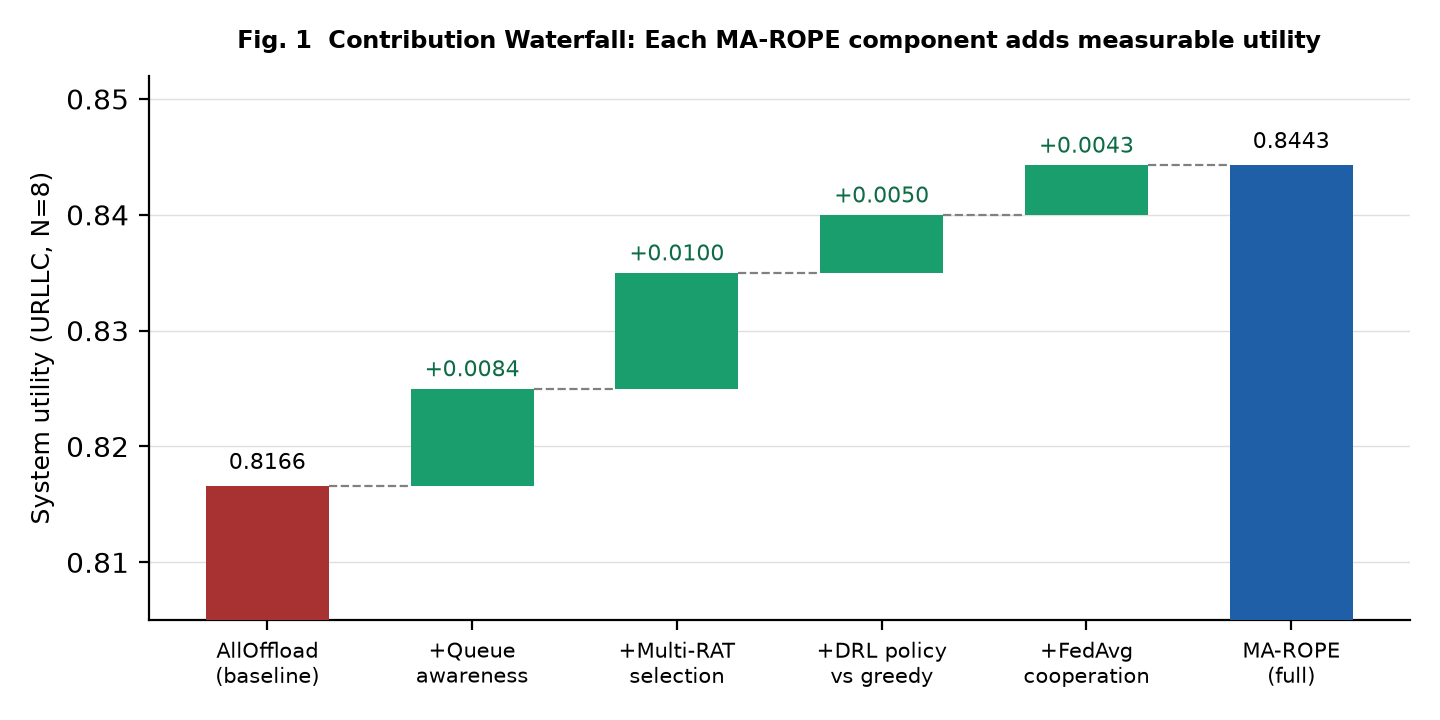
\includegraphics[width=0.45\textwidth]{figures/image2.png}
\caption{Contribution waterfall (URLLC, N=8 reference). AllOffload baseline (U=0.8166) to MA-ROPE full (U=0.8443): each component contributes independently.}
\label{fig:waterfall}
\end{figure}

\begin{figure}[htbp]
\centering
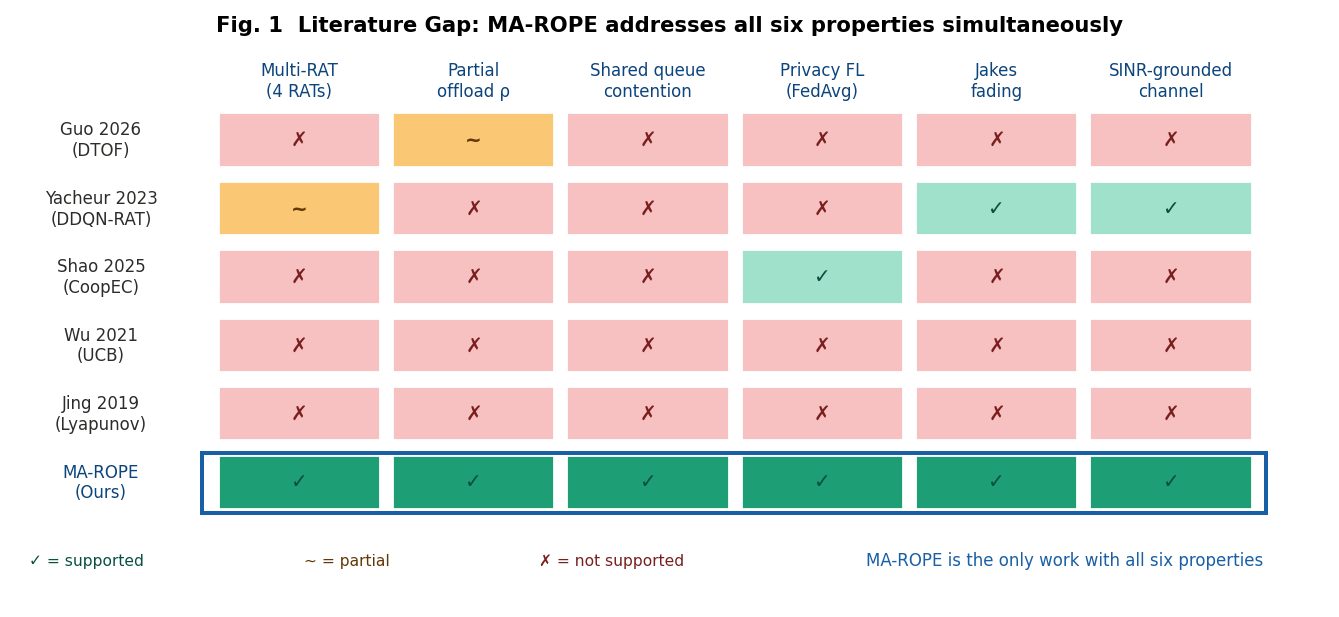
\includegraphics[width=0.45\textwidth]{figures/image1.png}
\caption{Literature gap matrix. MA-ROPE (bottom row, blue highlight) is the only framework with all six properties: supported, partial, or not supported.}
\label{fig:gap_matrix}
\end{figure}
